\section{IWR6843 Radar Interface and Configuration}
\label{sec:IWR6843 Radar Interface and Configuration}
The IWR6843AOPEVM development board from Texas Instruments features the IWR6843AOP, a high performance 4D mmWave FMCW sensor with Antenna On Package (AOP) design.
Although IWR6843AOP is intended for industrial applications and its complementary chip, AWR6843AOP, for automotive applications, IWR6843AOP was used in this project because it is available in the form of this development board and the two chips are identical in terms of their functionalities, only differing in compliance with automotive  industry \cite{iwr_awr_diff}.
Its small physical size, due to its AOP design, makes it an optimal choice for the desired mounting position, the go-kart's steering column.
\begin{figure}[!htbp]
    \centering
    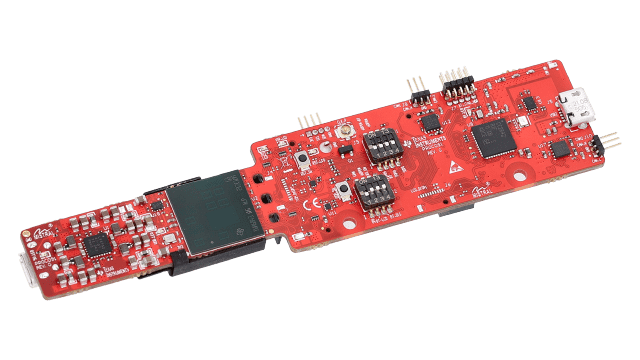
\includegraphics[width=0.7\linewidth]{images/iwr6843aopevm-angled.png}
    \caption{IWR6843AOP sensor\\
    \textit{Source: Texas Instruments, available at \url{https://www.ti.com/ds_dgm/images/fbd_swrs219f.gif}}}
    \label{fig:IWR6843AOP sensor}
\end{figure}
\par
The IWR6843AOP radar sensor operates within the frequency range of \SIrange{60}{64}{\giga\hertz} and integrates 4 receive (RX) and 3 transmit (TX) antennas, radio frequency (RF) front-end stages, analog signal processing, and digital signal processing (DSP).
It offers a wide range of communication interfaces including SPI, I2C, CAN-FD, UART and LVDS for raw data access and an Arm Cortex-R4F microcontroller for user-applications \cite{dev_board_page}.

\begin{figure}[!htbp]
    \centering
    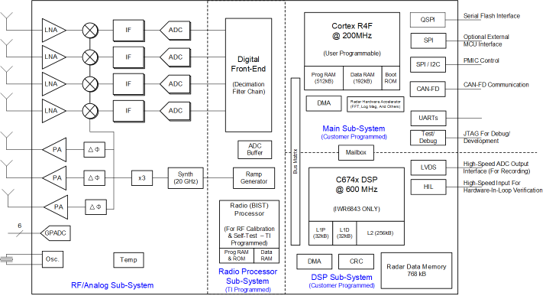
\includegraphics[width=1.0\linewidth]{images/blockdiagram.png}
    \caption{IWR6843AOP internal block diagram.\\
    \textit{Source: Texas Instruments, available at \url{https://www.ti.com/ds_dgm/images/fbd_swrs219f.gif}}}
    \label{fig:IWR6843AOP_internal}
\end{figure}

\FloatBarrier\noindent
Texas Instruments offers various demo applications for the development board that utilize the internal microcontroller for showcasing the radar sensor's capabilities in different specialized scenarios.
It was found out that most of them only use the radar sensor itself only for obtaining a point cloud, which points include spatial information in form of $x,y,z$ coordinates and a radial speed information (the prior mentioned four dimensions of the sensor).
Application-specific processing of the point cloud itself is executed on an external computation device.
\par
The main demo application ("mmWave SDK demo") allows a versatile customization of the radar sensor's operating parameters and its discrimination capabilities while outputting the point cloud via its UART interface, accessible via the on-board USB to UART converter.
Although the demo seems to be intended to be used only for demonstration purposes, many projects based on Texas Instruments' mmWave radar sensors utilize it, because it poses a generic solution for obtaining (close to) real-time point cloud data from the sensor without prior development of a custom user-application for the radar sensor's internal microcontroller.
This setup was therefore chosen for supplying the emergency braking system with data.

\subsection{Utilizing the mmWave SDK demo}
The "mmWave SDK demo" was developed by Texas Instruments for showcasing the abilities of their mmWave radar sensors.
It consists of the radar sensor itself, supplying close to real-time point cloud data and an online tool for visualization of the raw output data and for the creation of a sequence of commands used for configuration of the radar sensor's operating parameters and output \cite{mmwave_demo_doc}.
Due to the demo's simple structure and the radar sensor's generic output, the online application can be replaced by a custom application replicating the online tool's behavior for making use of the data.
\par
In the demo application, the radar sensor opens two UART connections.
One connection is bidirectional at a lower speed of \SI{115200}{\baud} which is used to configure the radar sensor by sending the previously mentioned sequence of commands. 
The second connection is unidirectional, from the radar sensor to the receiver, at a higher speed of \SI{921600}{\baud} and is used for outputting a constant data stream after the radar sensor received its configuration and a start command.
As the data packets are encoded in a proprietary format and therefore need to be parsed prior to further processing, a custom software module was written in C++ and later ported to Python.
The module handles the radar sensor's setup by sending a configuration file containing the sequence of initialization commands and the cyclic parsing of the encoded data packets.
The sequence of commands was generated with Texas Instruments' online tool, as it provided graphical feedback while making the necessary compromises involved in setting up the radar sensor's operating parameters.

\subsection{Sensor Data Output Format}
As the data packets, containing the individual frames, are encoded in a proprietary format, they need to be parsed to allow for further processing.
Each frame starts with a frame header and contains a number of TLVs (Type, Length, Value) in which the actual payload data is stored\cite{mmwave_demo_doc}.
\begin{figure}[!htbp]
    \centering
    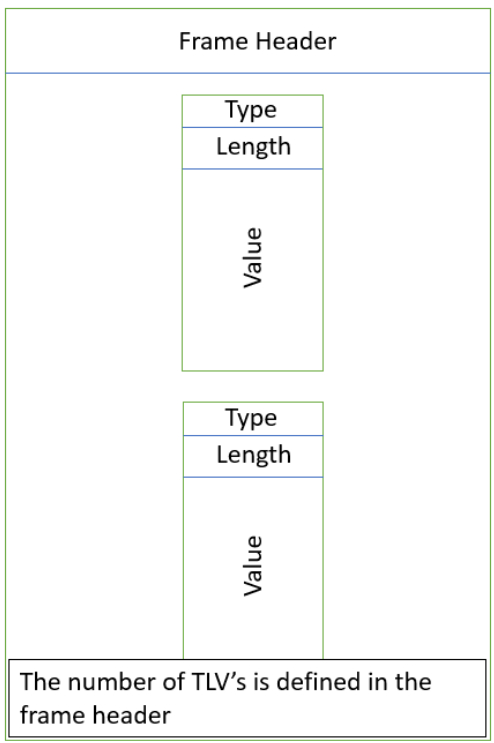
\includegraphics[width=0.4\linewidth]{images/UARTFrame.png}
    \caption{Frame structure. From \cite{mmwave_demo_output}.\\
    \textit{Source: Texas Instruments, available at \url{https://dev.ti.com/tirex/content/radar_toolbox_2_20_00_05/docs/software_guides/Understanding_UART_Data_Output_Format.html}}}
    \label{fig:UART data output format}
\end{figure}
\FloatBarrier\noindent
The frame's header has a total length of \SI{40}{\byte} and starts with a fixed magic word that denotes the start of each frame.
It also provides several other information in addition to the total packet length in bytes which is used to find the frame's end:
\begin{itemize}
    \item Magic Word: This value indicates the start of a new header, meaning that it can be used as a starting point for processing each frame.
    \item Total Packet Length: Total number of bytes in the frame (including the header) which can be used to calculate the frame's end.
    \item Platform: Indicates the device type and can be used for validating the radar sensor type. In the case of the device used for this project (IWR6843AOP) the expected value is "$0xA6843$".
    \item Number of TLVs: Total number of TLV's that exist in that specific frame.
\end{itemize}
\begin{figure}[!htbp]
    \centering
    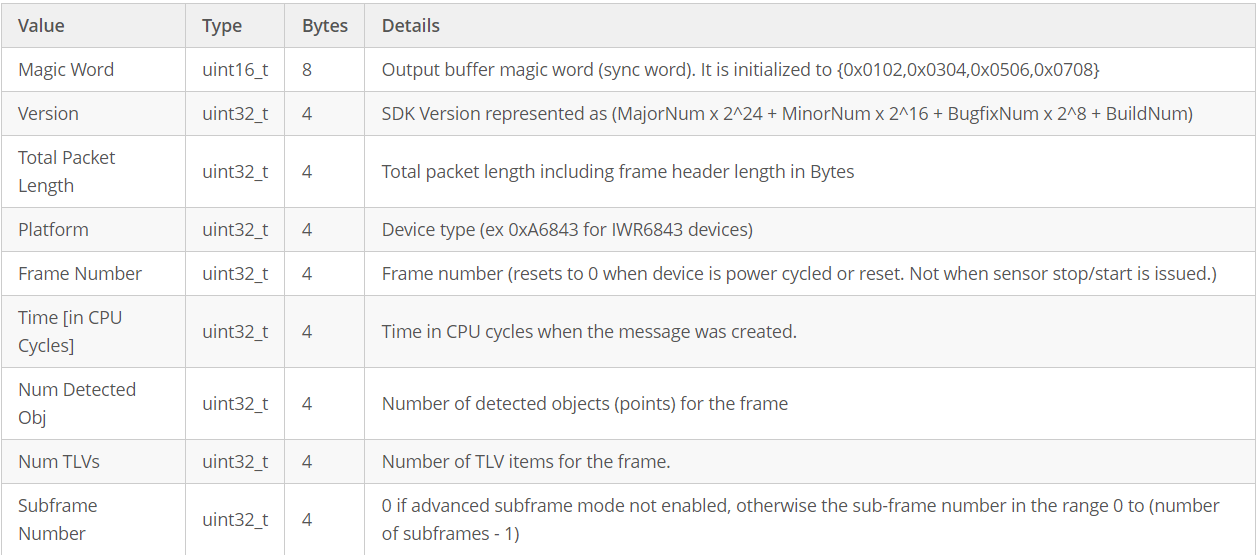
\includegraphics[width=1.0\linewidth]{images/FrameFormatHeader.png}
    \caption{Frame header format. From \cite{mmwave_demo_output}.\\
    \textit{Source: Texas Instruments, available at \url{https://dev.ti.com/tirex/content/radar_toolbox_2_20_00_05/docs/software_guides/Understanding_UART_Data_Output_Format.html}}}
    \label{fig:Frame header format}
\end{figure}
\FloatBarrier\noindent
The frame contains one or more TLVs after its header.
Each TLV has a header itself in which it specifies its length and which type of data (point cloud, doppler heatmaps, statistics, ...) is contained inside.
Each TLV type needs to be decoded differently, as it represents a different type of data.
\begin{figure}[!htbp]
    \centering
    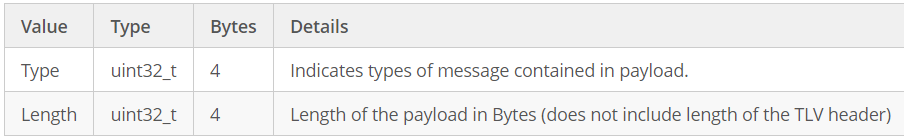
\includegraphics[width=0.95\linewidth]{images/TLVHeader.png}
    \caption{TLV header format. From \cite{mmwave_demo_output}.\\
    \textit{Source: Texas Instruments, available at \url{https://dev.ti.com/tirex/content/radar_toolbox_2_20_00_05/docs/software_guides/Understanding_UART_Data_Output_Format.html}}}
    \label{fig:TLV header format}
\end{figure}
\FloatBarrier

\subsection{Sensor-Tuning}
As some operating parameters influence each other, their selection must be done carefully while observing the influence of the trade-offs involved.
This could be referred to as "sensor tuning" and is a critical step because it directly impacts the system's accuracy and performance.

The following operating parameters can be tuned:
\begin{itemize}
    \item Frame rate
    \item Range resolution
    \item Maximum unambigious range
    \item Maximum radial velocity
    \item Radial velocity resolution
\end{itemize}

Tuning these operating parameters introduces trade-offs by influencing each other in the following ways:
\begin{table}[h]
    \centering
    \resizebox{\columnwidth}{!}{
    \begin{tabular}{|l|l|p{3.5cm}|p{3.5cm}|p{3.5cm}|}
        \hline
        \textbf{Tuning Parameter} & \textbf{Effect on Performance} & \textbf{Related HW Block} & \textbf{Trade-Off} \\
        \hline
        Frame Rate & Higher FPS = faster updates but more processing load & C674x DSP, Radar Data Memory & Higher FPS reduces maximum range \\
        \hline
        Range Resolution & Higher resolution = better object separation & ADC, 1D FFT (Range FFT) & Higher resolution reduces max range \\
        \hline
        Maximum Range & Determines farthest detectable object & RF Front-End, PA, LNA, ADC & Higher range lowers resolution \\
        \hline
        Radial Velocity Resolution & Improves speed accuracy & DSP, 2D FFT (Doppler FFT) & Higher resolution requires more chirps \\
        \hline
        Maximum Radial Velocity & Detects fast-moving objects & Chirp rate, TX Antennas, 2D FFT & Higher max velocity reduces resolution \\
        \hline
    \end{tabular}
    }
    \caption{Radar System Tuning Parameters and Trade-offs}
    \label{tab:mmWave_Sensor_Parameters}
\end{table}
The resulting overall accuracy of the velocity and distance measurements is again dependent on these operating parameters:
\begin{itemize}
\item \textbf{Radial velocity accuracy:} A fine balance between velocity resolution and frame rate must be maintained to ensure precise Doppler shift measurements. Lower resolution results in rounded velocity values, while an excessively high frame rate may introduce computational bottlenecks.
\item \textbf{Distance accuracy:} Optimizing range resolution and maximum range ensures that detected objects are positioned accurately within the environment. Increasing range often sacrifices resolution, leading to potential inaccuracies in close-range detections.
\item \textbf{Signal processing considerations:} The FFT calculation parameters directly affect both range and Doppler calculations, influencing the ability to distinguish between objects and detect small velocity variations.
\end{itemize}

This shows that finding exact values for the operation parameters by adjusting them while carefully watching their influences is crucial and heavily dependent on the particular application.
The test scenario required a frame rate of approximately 30Hz to balance responsiveness and computational load, together with sufficient range and velocity coverage to capture typical vehicle dynamics.

The resulting configuration yielded the following operating parameters:
\begin{itemize}
\item Frame rate: \SI{30}{\frame\per\second}
\item Range resolution: \SI{0.047}{\meter}
\item Maximum unambiguous range: \SI{9.78}{\meter}
\item Maximum radial velocity: \SI{8.01}{\meter\per\second}
\item Radial velocity resolution: \SI{0.51}{\meter\per\second}
\end{itemize}

Tuning and choosing the sensor's parameters carefully is extremely important as it defines the accuracy of 
therefore influences the reliability of the entire radar system.
Fine-tuning these settings ensures that the sensor operates optimally, enabling more precise self-speed estimation and overall system performance.
The accuracy of radial speed estimation and distance measurements depends directly on the tuning of these parameters. A poorly configured sensor can result in erroneous velocity estimations, unreliable object detection, or excessive noise in Doppler measurements. 
An example of the influence of the selection of the correct parameters on the output point cloud of the radar sensor can be found in Fig.~\ref{fig:IWR6843AOP Calibration example2 for the sensor}.

\begin{figure}[!htbp]
    \centering
    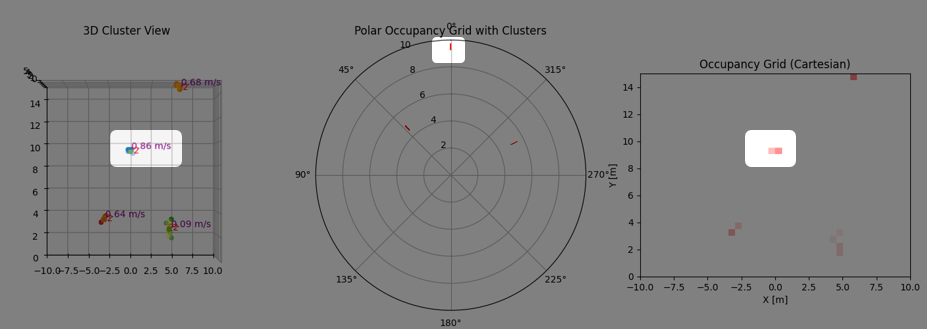
\includegraphics[width=1.0\linewidth]{images/calib_ex.png}
    \caption{Output of the IWR6843AOP prior sensor tuning.}
    \label{fig:IWR6843AOP Calibration example for the sensor}
\end{figure}

\begin{figure}[!htbp]
    \centering
    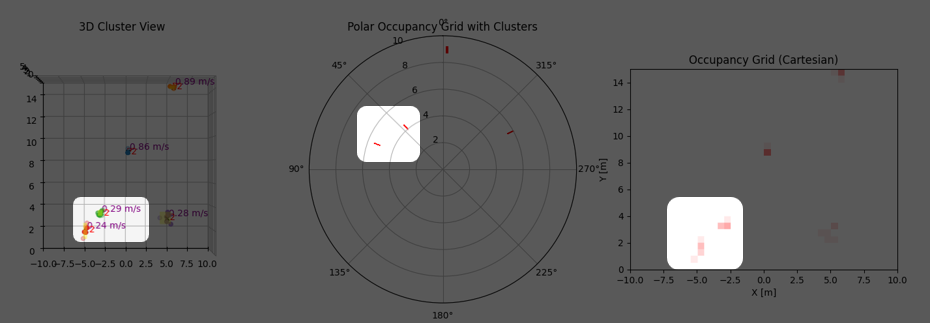
\includegraphics[width=1.0\linewidth]{images/calib_ex2.png}
    \caption{Output of the IWR6843AOP after sensor tuning.}
    \label{fig:IWR6843AOP Calibration example2 for the sensor}
\end{figure}

\subsection{Dual Sensor-Tuning} 
In addition to the individual calibration of each radar, further adjustments were required to enable a dual-sensor configuration with overlapping fields of view. 
The sensors were physically rotated around the $Z$-axis to widen the horizontal coverage and tilted by $15^\circ$ around the $X$-axis to prevent ground reflections and reduce clutter in the point clouds. 

\subsubsection{Chirp Calibration with Frequency Shift} 
Although both sensors operated under the same high-level parameters, their chirps had to be tuned to avoid mutual interference and ghost detections. 
To achieve this, each radar was configured to occupy only 2\,GHz of the available 4\,GHz bandwidth, introducing a frequency shift between the sensors. 
The resulting chirp design was derived using the Texas Instruments \textit{mmWave Sensing Estimator} tool \cite{understanding_uart}, which provides interactive validation of scene-dependent parameters, chirp design, and power consumption estimates. 
This configuration allowed the sensors to operate simultaneously without cross-talk while maintaining sufficient range resolution and velocity accuracy. 

\subsubsection{Geometric Transformations} 
To merge both radar outputs into a consistent reference frame, rigid-body transformations were applied to compensate for rotation, tilt, and translation offsets between the sensors. 
Each radar detections were first processed in its local coordinate frame and then transformed into the vehicle-centric frame before fusion into a single point cloud. 

Figures~\ref{fig:dualSensorCalib_rawComparison}--\ref{fig:dualSensorCalib_RANSACComparison} illustrate the effect of this calibration process at different processing stages: 
\begin{itemize} 
    \item \textbf{Raw point clouds:} Before calibration (Fig.~\ref{fig:dualSensorCalib_rawComparison}a), the detections from each sensor appear misaligned, producing duplicated landmarks. After applying the transformations (Fig.~\ref{fig:dualSensorCalib_rawComparison}b), both perspectives are fused into a coherent scene. 
    \item \textbf{Clustered view:} When clustering is applied, the uncalibrated data (Fig.~\ref{fig:dualSensorCalib_clusterComparison}a) shows inconsistent cluster centers, while the calibrated version (Fig.~\ref{fig:dualSensorCalib_clusterComparison}b) produces compact and aligned clusters. 
    \item \textbf{RANSAC Doppler fitting:} Similarly, Doppler–azimuth consistency improves after calibration. Uncalibrated detections (Fig.~\ref{fig:dualSensorCalib_RANSACComparison}a) yield noisier distributions, while the calibrated outputs (Fig.~\ref{fig:dualSensorCalib_RANSACComparison}b) produce smoother fits with fewer outliers. 
\end{itemize} 

The transformed data thus provides a coherent and stable input for the odometry estimation pipeline, ensuring that static landmarks are consistently aligned across both sensors.  

\begin{figure}[ht]
    \centering
    \begin{subfigure}[b]{0.45\textwidth}
        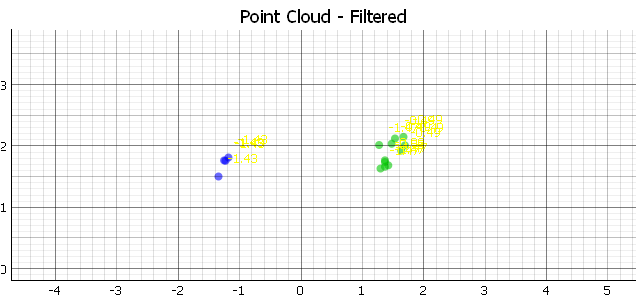
\includegraphics[width=\textwidth]{images/dualSensorCalib_2mts.png}
        \caption{Raw point cloud before calibration}
    \end{subfigure}
    \hfill
    \begin{subfigure}[b]{0.45\textwidth}
        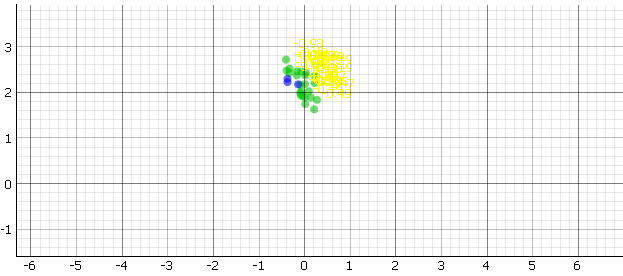
\includegraphics[width=\textwidth]{images/AFTERdualSensorCalib_2mts.png}
        \caption{Raw point cloud after calibration}
    \end{subfigure}
    \caption{Dual-sensor raw detections before and after applying geometric transformations.}
    \label{fig:dualSensorCalib_rawComparison}
\end{figure}

\begin{figure}[ht]
    \centering
    \begin{subfigure}[b]{0.3\textwidth}
        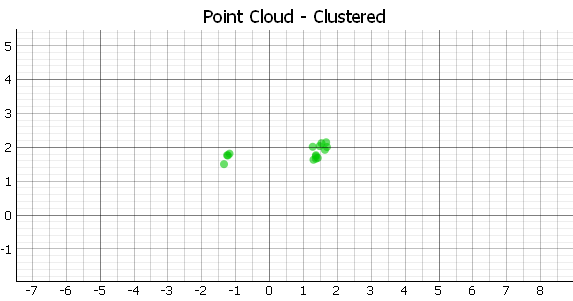
\includegraphics[width=\textwidth]{images/dualSensorCalibCluster_2mts.png}
        \caption{Clustered detections before calibration}
    \end{subfigure}
    \hfill
    \begin{subfigure}[b]{0.3\textwidth}
        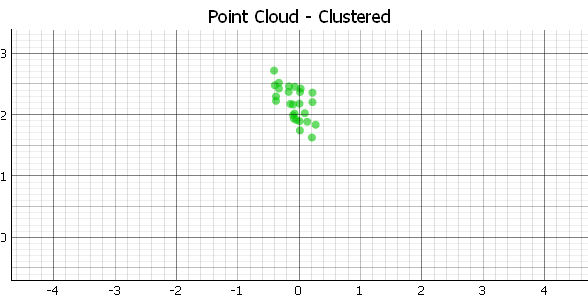
\includegraphics[width=\textwidth]{images/AFTERdualSensorCalibCluster_2mts.png}
        \caption{Clustered detections after calibration}
    \end{subfigure}
    \caption{Effect of calibration on cluster alignment across sensors.}
    \label{fig:dualSensorCalib_clusterComparison}
\end{figure}

\begin{figure}[ht]
    \centering
    \begin{subfigure}[b]{0.3\textwidth}
        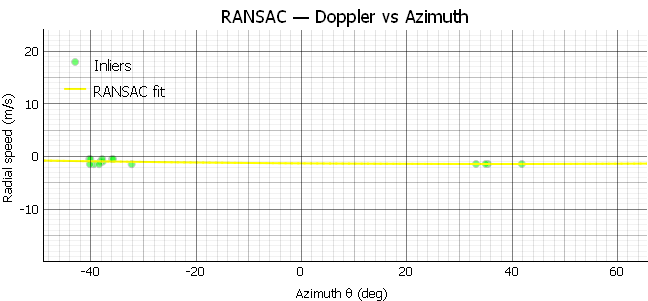
\includegraphics[width=\textwidth]{images/dualSensorCalibRANSAC_2mts.png}
        \caption{RANSAC Doppler fitting before calibration}
    \end{subfigure}
    \hfill
    \begin{subfigure}[b]{0.3\textwidth}
        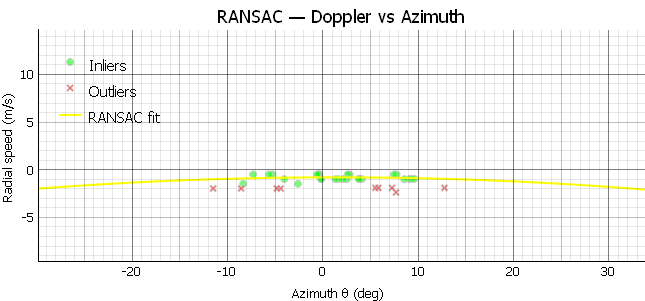
\includegraphics[width=\textwidth]{images/AFTERdualSensorCalibRANSAC_2mts.png}
        \caption{RANSAC Doppler fitting after calibration}
    \end{subfigure}
    \caption{Improvement in Doppler-azimuth consistency after calibration.}
    \label{fig:dualSensorCalib_RANSACComparison}
\end{figure}

\FloatBarrier